\documentclass[12pt]{article}
\usepackage[utf8]{inputenc}
\usepackage{hyperref}
\usepackage{times}
\usepackage{graphicx}
\graphicspath{ {./} }
\usepackage[toc,page]{appendix}
\usepackage{pgffor}

\title{Exploration of jet substructure with \\ Energy Flow Polynomials}
\author{Yu-Heng Yu\\
\normalsize{CERN Summer Student 2019}\\
\normalsize{Supervisors: Kirill Lapidus, Nima Zardoshti}\\
\normalsize{Contact: yu-heng.yu@cern.ch}\\
}

\date{}

\newenvironment{sciabstract}{%
\begin{quote} \bf}
{\end{quote}}

\topmargin 0.0cm
\oddsidemargin 0.2cm
\textwidth 16cm 
\textheight 22cm
\footskip 1.0cm
\usepackage{amsmath}

\begin{document}

\maketitle

\begin{sciabstract}
The Energy Flow Polynomials (EFPs) are a set of jet substructure observables which forms an overcomplete basis for all infrared- and collinear-safe observables. In this study, an in-depth look into the EFPs is conducted. Comparisons of EFPs distributions are made between experimental and simulated dataset; strong correlations between different EFPs are found; Principal Component Analysis is done to 53 different EFPs, where they can be reduced to 6 Principal Axes without much loss of information; Linear Regression is done to the same set of EFPs, and also to the 6 reduced axes, to find the coefficients for them to linearly combine into some traditional jet shapes. Similar performance are found between the 53 EFPs and the 6 Principal Axes.
\end{sciabstract}
\section{Introduction}
% The EFPs are a set of jet substructure observables \cite{EFP} which one can calculate for a jet using some energy and angle information of the jet's constituents. They are an \emph{over}complete basis for all infrared- and collinear-safe (IRC safe) observables, meaning that any IRC safe observables of a jet can be constructed by linear combining the EFPs of that jet, and that one can dismiss at least one EFP without affecting the completeness of this basis.

% It is then interesting to have a more detailed look into the EFPs and study the relations between different EFPs, by which one can see strong correlations between different EFPs. For a set of data that has strongly correlated basis, one can choose a new set of basis such that the first component has the largest possible variance, making it contain the most information of the dataset, and each succeeding component has the highest variance possible under the constraint that it is orthogonal to the preceding components. This process of choosing a new basis is call Principal Component Analysis (PCA), by which we can choose the first few Principal Component, hence reducing the dimension of the basis. After dimensionality reduction, it is important to see if the reduced basis has the same ability to linearly combine into IRC-safe observables.

% \section{Energy Flow Polynomials}
% In this section, the formula and graphic representations of EFPs are introduced, then comparisons are made for some EFP distributions between an experimental and a simulated dataset. Finally, correlations between different EFPs are shown using the experimental dataset.
% \subsection{Formula and Graphic Representation}
% From ref. \cite{EFP} (page.2) one can see how the EFPs are defined, and how they can be represented by multigraphs:
% \begin{quote}
% There is a one-to-one correspondence between EFPs and loopless multigraphs, which
% helps to visualize and calculate the EFPs. A multigraph is a graph where any two vertices can be connected by multiple edges; in this context, a \emph{loop} is an edge from a vertex to itself, while a closed chain of edges is instead referred to as a cycle. For a multigraph $G$ with $N$ vertices and edges $(k,l) \in G$, the corresponding EFP takes the form:
% \begin{equation}\label{eq:EFP}
% \text{EFP}_G = \sum_{i_1=1}^M \cdot\cdot\cdot \sum_{i_N=1}^M z_{i_1} \cdot\cdot\cdot z_{i_N} \prod_{(k,l)\in G} \theta _{i_ki_j}
% \end{equation}
% where the jet consists of $M$ particles, $z_i \equiv E_i/\sum_{j=1}^{M}E_j$ is the energy fraction carried by particle $i$, and $\theta_ij$ is the angular distance between particles $i$ and $j$. The precise definitions of $E_i$ and $\theta_ij$ will depend on the collider context.
% \end{quote}
% This can be graphically shown as below:
% \begin{equation}\label{eq:graph}
% 
\includegraphics[width=3mm]{00.png}_j \Longleftrightarrow \sum_{{i_j}=1}^M z_{i_j}, \ \ \ \ \  k \ 
\includegraphics[width=20mm]{01.png} \ l \Longleftrightarrow \theta_{i_ki_l}
% \end{equation}
% As an example:

% \newcommand{\vcenteredinclude}[1]{\begingroup
% \setbox0=\hbox{\includegraphics[width=22mm]{#1}}%
% \parbox{\wd0}{\box0}\endgroup}

% \begin{equation}\label{eq:graph_ex}
% \ \vcenteredinclude{31.png} \ = \ \sum_{i_1=1}^M\sum_{i_2=1}^M\sum_{i_3=1}^M\sum_{i_4=1}^M z_{i_1}z_{i_2}z_{i_3}z_{i_4} \theta_{i_1i_2}\theta_{i_2i_3}\theta_{i_2i_4}^2\theta_{i_3i_4}
% \end{equation}

% In this study, the datasets used are from hadronic collisions, which by ref. \cite{EFP}, the energy in \eqref{eq:EFP} is defined as the transverse momentum, and the $\theta_{ij}$ is defined as:
% \begin{equation}\label{eq:theta}
% \theta_{ij} = (\Delta y_{ij}^2 +\Delta \phi_{ij}^2)^{\beta/2}
% \end{equation}
% where $\Delta y_{ij} \equiv y_i - y_j$, $\Delta \phi_{ij} \equiv \phi_i - \phi_j$ are determined by the rapidity $y_i$ and azimuth $\phi_i$ of particle $i$. The angular exponent $\beta$ can take on any positive value and still be consistent with IRC safety, and it is set to be 1 in this study.

% The python package EnergyFlow is used for calculating the EFPs.

% \subsection{EFP Distributions}
% In this section, EFP distributions are plotted using an 2013 ALICE experimental dataset of p-Pb collisions at 5 TeV (exp data) against a Monte Carlo simulated dataset of PYTHIA6 p-p collisions at 5 TeV (MC), with $R=0.4$ charged jets clustered with anti-kt algorithm. Both exp data and MC are at the detector level. Since the transverse momentum ($p_T$) distribution of the MC was different from that of the exp data originally, it was manually fitted to the exp data so that they have the same $p_T$ distribution (fig.\ref{fig:pt})
% \begin{figure}[h]
% \begin{center}
% 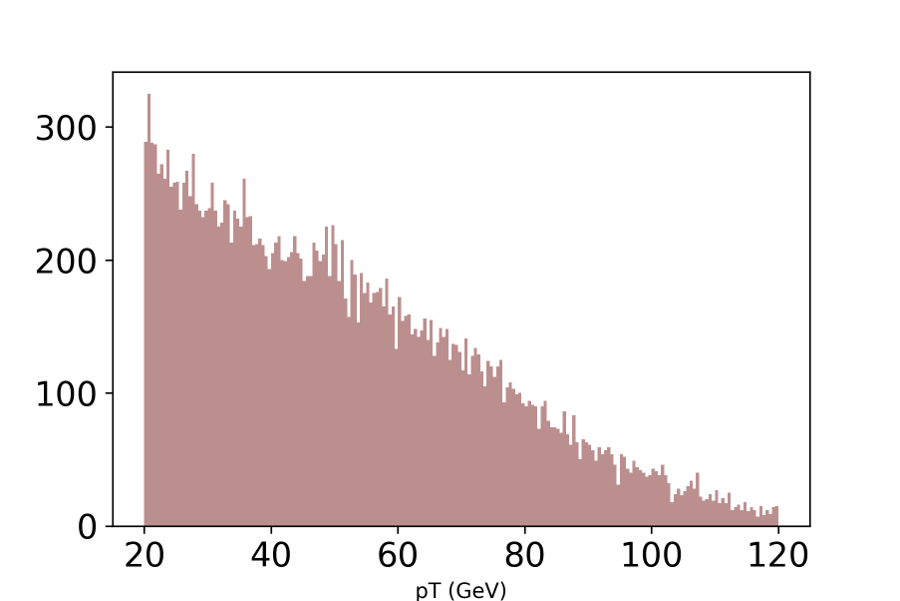
\includegraphics[width = 75mm]{ptMC.png}
% 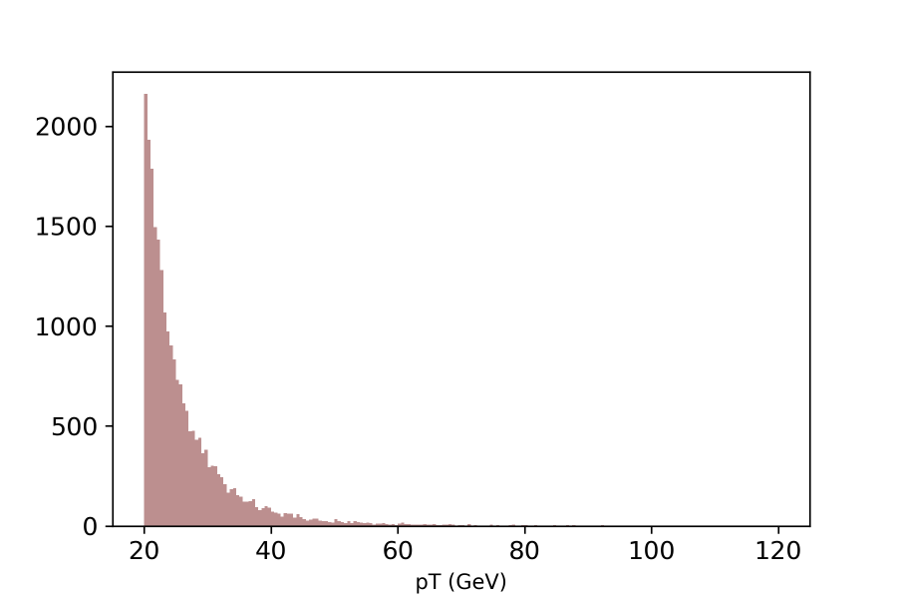
\includegraphics[width = 75mm]{ptEXP.png}
% \caption{$p_T$ distributions of MC (left) and exp data (right)}
% \label{fig:pt}
% \end{center}
% \end{figure}

% First we select only the jets with $20 \ GeV < p_T < 120 \ GeV$, then the $p_T$ distributions of the jets are plotted with $ bin \ width = 0.5 \ p_T$. The ratio of the $bin \ height$ of the MC to that of the exp data are then calculated for each bin, denoted as $w(p_T)$. To plot the distributions of an EFP using the MC, the EFP for each jet $j$ is calculated and filled to a histogram with weight $w({p_T}_j)$.

% Only 53 EFPs, as shown by the multigraphs in appendix \ref{appendix:all_EFP}, are analyzed in this study. Only 4 are shown in fig.\ref{fig:EFP_basis}, while all of them are shown in appendix \ref{appendix:EFP_basis}.

% \newcommand{\basis}[1] {
% \includegraphics[width = 38mm]{basis_mc_ptscaled/{#1}.png}
% }
% \begin{figure}[htbp]
% \begin{center}
% \basis{0}\basis{1}\basis{2}\basis{3}
% \caption{MC and exp data comparison for EFP distributions, $20 \ GeV < p_T < 120 \ GeV$}
% \label{fig:EFP_basis}
% \end{center}
% \end{figure}

% A generally good agreement of the EFP distributions between MC and exp data can be seen. To take the analysis further, the same comparisons is done for finer $p_T$ selections ($20 \ GeV < p_T \leq 30 \ GeV$, $30 \ GeV < p_T \leq 40 \ GeV$, $40 \ GeV < p_T \leq 50 \ GeV$) as shown in fig.\ref{fig:EFP_basis_pt}.
% Only 4 EFPs are shown, while one can refer to appendix \ref{appendix:EFP_basis} for the distributions for all 53 EFPs.

% \newcommand{\basispt}[2] {
% \includegraphics[width = 38mm]{basis_mc_pt_ptscaled/{#1}/{#2}.png}
% }
% \begin{figure}[t]
% \begin{center}
% \basispt{0}{0}\basispt{0}{1}\basispt{0}{2}\basispt{0}{3}
% \basispt{1}{0}\basispt{1}{1}\basispt{1}{2}\basispt{1}{3}
% \basispt{2}{0}\basispt{2}{1}\basispt{2}{2}\basispt{2}{3}
% \caption{MC and exp data comparison for EFP distributions, $20 \ GeV < p_T \leq 30 \ GeV$ (top), $30 \ GeV < p_T \leq 40 \ GeV$ (middle), $40 \ GeV < p_T \leq 50 \ GeV$ (bottom)}
% \label{fig:EFP_basis_pt}
% \end{center}
% \end{figure}

% One can see that at lower $p_T$ region the differences between the MC and the exp data are small. However, the differences grow for higher $p_T$. Further investigation is required to understand this effect.

% \subsection{Correlations Between Different EFPs}
% The correlations between different EFPs are examined by plotting 2-dimensional plots, where in each plot one EFP act as the x-axis, and another one act as the y-axis. The EFPs are chosen randomly for the comparison, fig.\ref{fig:2D} shows 4 of them, while in appendix \ref{appendix:2D}, 15 of them are shown, where one can see that the EFPs are strongly correlated. From all content below only exp data are used.
% \newcommand{\twoD}[2] {
% \includegraphics[width = 38mm]{2D/#1_#2.png}
% }
% \begin{figure}[htbp]
% \begin{center}
% \twoD{10}{35}\twoD{14}{16}\twoD{1}{5}\twoD{20}{25}
% \caption{2D EFP plots}
% \label{fig:2D}
% \end{center}
% \end{figure}

% \section{Principal Component Analysis on the EFPs}
% \subsection{Principal Component Analysis}
% Principal Component Analysis (PCA) is a statistical procedure that uses orthogonal transformation to choose a new set of basis called principal components, which the first principal component has the largest possible variance, and each succeeding component has the highest variance possible under the constraint that it is orthogonal to the preceding components. In this study, PCA is performed using the python package Scikit-learn.

% One can perform PCA on a dataset, and reduce the dimension of the dataset by taking the first few principal components and project the dataset onto them. This would surely cause some lost of information, however, for a dataset that has its basis strongly correlated, the lost would be small. To illustrate this, in fig.\ref{fig:PCAexco} PCA were performed on a 2D dataset whose basis is strongly correlated. The distribution of the dataset on one of the axes are compared before and after PCA. The same are done for an uncorrelated dataset in fig./ref{fig:PCAexunco}. One can see that the distribution does not change much for correlated dataset, but is vastly different for the uncorrelated one.

% \begin{figure}[htb]
% \begin{center}
% 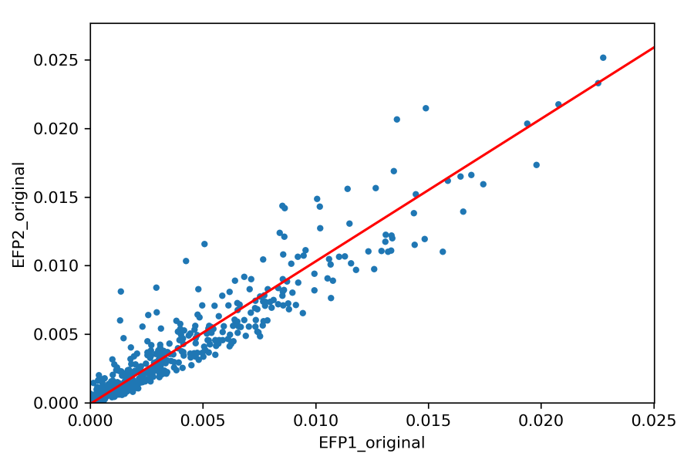
\includegraphics[width = 50mm]{PCAex_co_before.png}
% 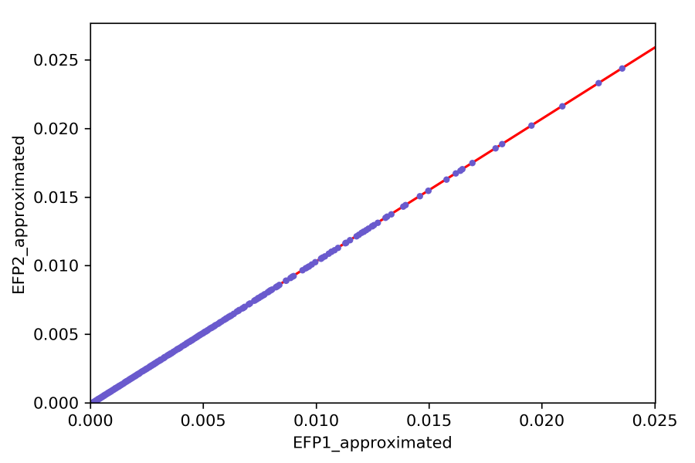
\includegraphics[width = 50mm]{PCAex_co_after.png}
% \\
% 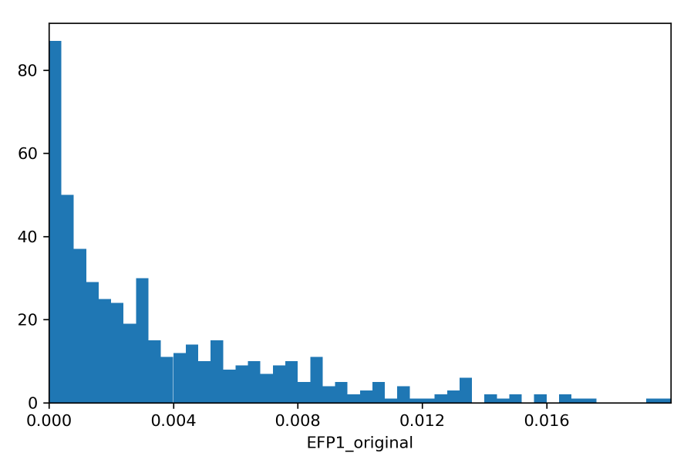
\includegraphics[width = 50mm]{PCAex_co_before_x.png}
% 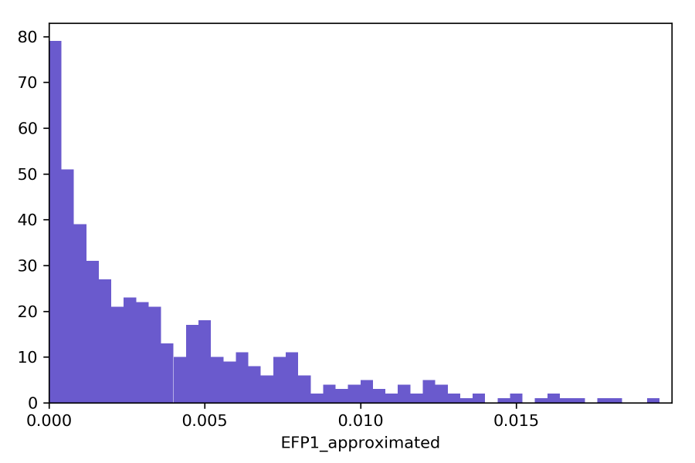
\includegraphics[width = 50mm]{PCAex_co_after_x.png}
% \begin{minipage}{0.65\textwidth} 
% {\footnotesize PCA is done to the original dataset in the top-left, where the red line denotes the first principal axis. Then the dataset were projected onto the first principal axis, so the dimension is reduced from two to one. The bottom two plots are the distribution of the dataset on the horizontal axis before (left) and after (right) the PCA\par}
% \end{minipage}
% \caption{An example of PCA on a correlated dataset}
% \label{fig:PCAexco}
% \end{center}
% \end{figure}
% \begin{figure}[htb]
% \begin{center}
% 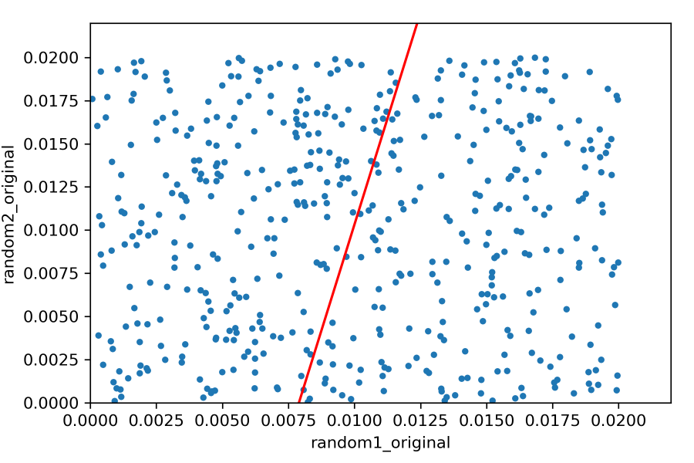
\includegraphics[width = 50mm]{PCAex_unco_before.png}
% 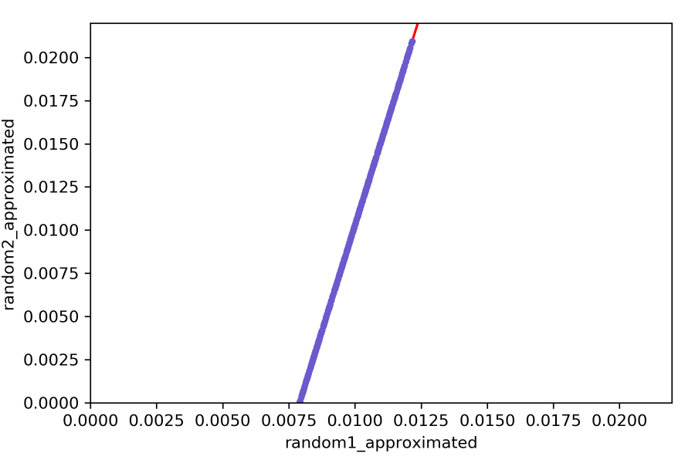
\includegraphics[width = 50mm]{PCAex_unco_after.png}
% \\
% 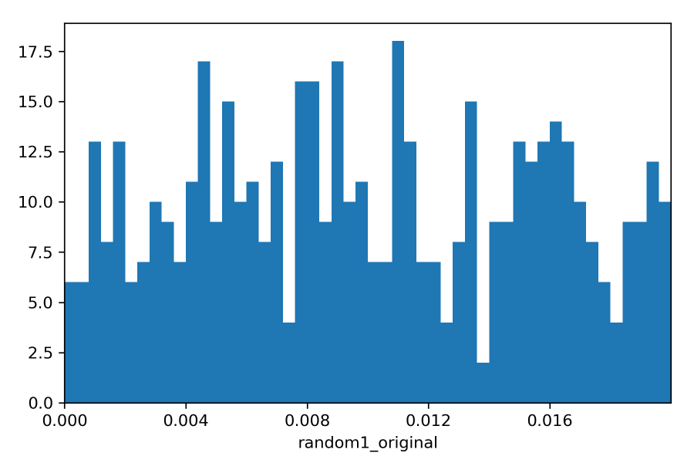
\includegraphics[width = 50mm]{PCAex_unco_before_x.png}
% 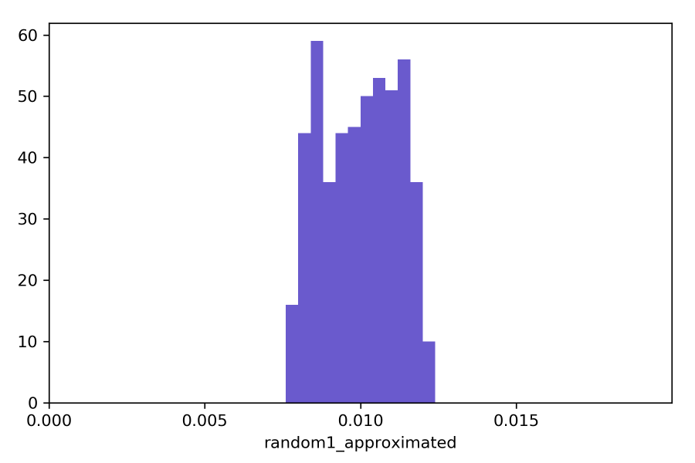
\includegraphics[width = 50mm]{PCAex_unco_after_x.png}
% \begin{minipage}{0.65\textwidth} 
% {\footnotesize The analysis procedure is the same as in fig.\ref{fig:PCAexco}\par}
% \end{minipage}
% \caption{An example of PCA on an uncorrelated dataset}
% \label{fig:PCAexunco}
% \end{center}
% \end{figure}

% \subsection{Dimension Reduction On The EFPs}
% For the examples in fig.\ref{fig:PCAexco} and fig.\ref{fig:PCAexunco} the dimension was only reduced from two to one; however, PCA allows us to reduce any dimension $m$ to $n$ where $1 \leq n \leq m$ using the same procedure. In fig.\ref{fig:PCA} PCA is done to the 53 EFPs, and they are reduced to 6 principal axes. The distribution of EFPs are plotted as in the examples. They are also plotted using only 1 principal axis (that is, the dimension is reduced to 1) for comparison. All 53 EFP distributions plotted using 6 reduced axes are shown in appendix \ref{appendix:PCA}. One can see that just by 6 principal axes, the 53 EFPs can be described fairly well.
% \newcommand{\PCA}[2] {
% \includegraphics[width = 38mm]{PCA/{#1}/{#2}.png}
% }
% \begin{figure}[htb]
% \begin{center}
% \PCA{1}{0}\PCA{1}{10}\PCA{1}{30}\PCA{1}{50}\\
% \PCA{6}{0}\PCA{6}{10}\PCA{6}{30}\PCA{6}{50}
% \begin{minipage}{0.65\textwidth} 
% {\footnotesize EFP distributions are plotted using the original dataset (original) and the dataset with dimension reduced to 1 (top) and 6 (bottom) using PCA (approx)\par}
% \end{minipage}
% \caption{EFP distributions of the dataset with PCA reduced dimension}
% \label{fig:PCA}
% \end{center}
% \end{figure}

\section{Decomposing Traditional Jet Observables Using EFPs}
By linearly combining the EFPs, one can get any IRC-safe jet observables. The coefficient of each EFP can be calculated as suggest in \cite{EFP}:


\clearpage
\begin{appendices}
% \section{All EFPs Analysed in This Study}
% \label{appendix:all_EFP}
% The multigraphs corresponding to all the EFPs analysed in this study are shown, where the $d$ in the figure denotes the number of edges of the multigraph.
% \begin{center}
% \includegraphics[width = 140mm]{all_graphs.png}
% \end{center}
% \newcommand{\basisall}[1] {
% \includegraphics[width = 30mm]{basis_mc_ptscaled/{#1}.png}
% }
% \newcommand{\basisptall}[2] {
% \includegraphics[width = 30mm]{basis_mc_pt_ptscaled/{#1}/{#2}.png}
% }
% \section{More EFP Distributions}
% \label{appendix:EFP_basis}
% All 53 EFP distributions of the exp data against MC, for jets of the whole jet $p_T$ range ($20 \ GeV < p_T < 120 \ GeV$), $20 \ GeV < p_T \leq 30 \ GeV$, $30 \ GeV < p_T \leq 40 \ GeV$, and $40 \ GeV < p_T \leq 50 \ GeV$ are shown 
% \begin{center}
% \basisall{0}\basisall{1}\basisall{2}\basisall{3}\basisall{4}
% \basisall{5}\basisall{6}\basisall{7}\basisall{8}\basisall{9}
% \basisall{10}\basisall{11}\basisall{12}\basisall{13}\basisall{14}
% \basisall{15}\basisall{16}\basisall{17}\basisall{18}\basisall{19}
% \basisall{20}\basisall{21}\basisall{22}\basisall{23}\basisall{24}
% \basisall{25}\basisall{26}\basisall{27}\basisall{28}\basisall{29}
% \basisall{30}\basisall{31}\basisall{32}\basisall{33}\basisall{34}
% \basisall{35}\basisall{36}\basisall{37}\basisall{38}\basisall{39}
% \basisall{40}\basisall{41}\basisall{42}\basisall{43}\basisall{44}
% \basisall{45}\basisall{46}\basisall{47}\basisall{48}\basisall{49}
% \basisall{50}\basisall{51}\basisall{52}
% \basisptall{0}{0}\basisptall{0}{1}\basisptall{0}{2}\basisptall{0}{3}\basisptall{0}{4}
% \basisptall{0}{5}\basisptall{0}{6}\basisptall{0}{7}\basisptall{0}{8}\basisptall{0}{9}
% \basisptall{0}{10}\basisptall{0}{11}\basisptall{0}{12}\basisptall{0}{13}\basisptall{0}{14}
% \basisptall{0}{15}\basisptall{0}{16}\basisptall{0}{17}\basisptall{0}{18}\basisptall{0}{19}
% \basisptall{0}{20}\basisptall{0}{21}\basisptall{0}{22}\basisptall{0}{23}\basisptall{0}{24}
% \basisptall{0}{25}\basisptall{0}{26}\basisptall{0}{27}\basisptall{0}{28}\basisptall{0}{29}
% \basisptall{0}{30}\basisptall{0}{31}\basisptall{0}{32}\basisptall{0}{33}\basisptall{0}{34}
% \basisptall{0}{35}\basisptall{0}{36}\basisptall{0}{37}\basisptall{0}{38}\basisptall{0}{39}
% \basisptall{0}{40}\basisptall{0}{41}\basisptall{0}{42}\basisptall{0}{43}\basisptall{0}{44}
% \basisptall{0}{45}\basisptall{0}{46}\basisptall{0}{47}\basisptall{0}{48}\basisptall{0}{49}
% \basisptall{0}{50}\basisptall{0}{51}\basisptall{0}{52}
% \basisptall{1}{0}\basisptall{1}{1}\basisptall{1}{2}\basisptall{1}{3}\basisptall{1}{4}
% \basisptall{1}{5}\basisptall{1}{6}\basisptall{1}{7}\basisptall{1}{8}\basisptall{1}{9}
% \basisptall{1}{10}\basisptall{1}{11}\basisptall{1}{12}\basisptall{1}{13}\basisptall{1}{14}
% \basisptall{1}{15}\basisptall{1}{16}\basisptall{1}{17}\basisptall{1}{18}\basisptall{1}{19}
% \basisptall{1}{20}\basisptall{1}{21}\basisptall{1}{22}\basisptall{1}{23}\basisptall{1}{24}
% \basisptall{1}{25}\basisptall{1}{26}\basisptall{1}{27}\basisptall{1}{28}\basisptall{1}{29}
% \basisptall{1}{30}\basisptall{1}{31}\basisptall{1}{32}\basisptall{1}{33}\basisptall{1}{34}
% \basisptall{1}{35}\basisptall{1}{36}\basisptall{1}{37}\basisptall{1}{38}\basisptall{1}{39}
% \basisptall{1}{40}\basisptall{1}{41}\basisptall{1}{42}\basisptall{1}{43}\basisptall{1}{44}
% \basisptall{1}{45}\basisptall{1}{46}\basisptall{1}{47}\basisptall{1}{48}\basisptall{1}{49}
% \basisptall{1}{50}\basisptall{1}{51}\basisptall{1}{52}
% \basisptall{2}{0}\basisptall{2}{1}\basisptall{2}{2}\basisptall{2}{3}\basisptall{2}{4}
% \basisptall{2}{5}\basisptall{2}{6}\basisptall{2}{7}\basisptall{2}{8}\basisptall{2}{9}
% \basisptall{2}{10}\basisptall{2}{11}\basisptall{2}{12}\basisptall{2}{13}\basisptall{2}{14}
% \basisptall{2}{15}\basisptall{2}{16}\basisptall{2}{17}\basisptall{2}{18}\basisptall{2}{19}
% \basisptall{2}{20}\basisptall{2}{21}\basisptall{2}{22}\basisptall{2}{23}\basisptall{2}{24}
% \basisptall{2}{25}\basisptall{2}{26}\basisptall{2}{27}\basisptall{2}{28}\basisptall{2}{29}
% \basisptall{2}{30}\basisptall{2}{31}\basisptall{2}{32}\basisptall{2}{33}\basisptall{2}{34}
% \basisptall{2}{35}\basisptall{2}{36}\basisptall{2}{37}\basisptall{2}{38}\basisptall{2}{39}
% \basisptall{2}{40}\basisptall{2}{41}\basisptall{2}{42}\basisptall{2}{43}\basisptall{2}{44}
% \basisptall{2}{45}\basisptall{2}{46}\basisptall{2}{47}\basisptall{2}{48}\basisptall{2}{49}
% \basisptall{2}{50}\basisptall{2}{51}\basisptall{2}{52}
% \end{center}

% \section{More correlation plots between different EFPs}
% \label{appendix:2D}

% \newcommand{\twoDall}[2] {
% \includegraphics[width = 30mm]{2D/#1_#2.png}
% }
% \begin{center}
% \twoDall{16}{32}\twoDall{1}{52}\twoDall{22}{23}\twoDall{25}{50}\twoDall{26}{31}
% \twoDall{26}{34}\twoDall{27}{32}\twoDall{29}{33}\twoDall{2}{51}\twoDall{31}{35}
% \twoDall{35}{45}\twoDall{36}{40}\twoDall{45}{50}\twoDall{4}{51}\twoDall{5}{50}
% \end{center}
\newcommand{\PCAall}[1] {
\includegraphics[width = 30mm]{PCA/6/{#1}.png}
}
\section{More EFP distributions with PCA reduced dimension = 6}
\label{appendix:PCA}
% \begin{center}
% \PCAall{0}\PCAall{1}\PCAall{2}\PCAall{3}\PCAall{4}
% \PCAall{5}\PCAall{6}\PCAall{7}\PCAall{8}\PCAall{9}
% \PCAall{10}\PCAall{11}\PCAall{12}\PCAall{13}\PCAall{14}
% \PCAall{15}\PCAall{16}\PCAall{17}\PCAall{18}\PCAall{19}
% \PCAall{20}\PCAall{21}\PCAall{22}\PCAall{23}\PCAall{24}
% \PCAall{25}\PCAall{26}\PCAall{27}\PCAall{28}\PCAall{29}
% \PCAall{30}\PCAall{31}\PCAall{32}\PCAall{33}\PCAall{34}
% \PCAall{35}\PCAall{36}\PCAall{37}\PCAall{38}\PCAall{39}
% \PCAall{40}\PCAall{41}\PCAall{42}\PCAall{43}\PCAall{44}
% \PCAall{45}\PCAall{46}\PCAall{47}\PCAall{48}\PCAall{49}
% \PCAall{50}\PCAall{51}\PCAall{52}
% \end{center}


\end{appendices}


\bibliographystyle{plain}
\bibliography{M335}

\end{document}
